\section{Applications in QCD}
There relatively few text books with explicit 1-loop QCD calculations.
We will use \fc in the following for re-doing the 1-loop selfenergy calculation
as presented in the Appendix of \cite{Muta}.

Furthermore examples of two-loop gluon and quark self energy calculaions in a general
covariant gauge are given. For those examples we will use the recursion algorithm
of Tarasov \cite{Tar96} as implemented in Tarcer \cite{tarcer} in order to reduce
all 2-loop integrals to mater integrals.

\subsection*{The 2-loop gluon selfenergy }

%
% this is *one* graph from the 2-loop gluon selfenergy.
% it is from the g2seoffshell.nb notebook
%
% unfortunately FeynArts does the momenta labelling all pretty stupid and Thomas Hahn does
% not answer on how to define momenta flow per topology ...
% so either FeynAmpDenominatorSimplify should be improved or the model file, i.e., the
% setting of M$LastGenericRules 
%
%

\dispSFinmath{
<<\Mvariable{HighEnergyPhysics`FeynCalc`}
}

\subsubsection*{The graphs}

\dispSFinmath{
\MathBegin{MathArray}{l}
\Muserfunction{Paint}[\Mvariable{inserts}=
    \Muserfunction{InsertFields}[\Mvariable{Rest}@\Muserfunction{CreateTopologies}[
        2,1\rightarrow 1,\Mvariable{ExcludeTopologies}\rightarrow \{\Mvariable{Internal}\}],  \\
\noalign{\vspace{0.555556ex}}
   \hspace{3.em} \{V[5]\}\rightarrow \{V[5]\},\Mvariable{InsertionLevel}\rightarrow \{\Mvariable{Generic}\},
   \Mvariable{GenericModel}->"FCQCDLorentz",  \\
\noalign{\vspace{0.555556ex}}
\hspace{3.em} \Mvariable{Model}\rightarrow "FCQCD"],
     \Mvariable{ColumnsXRows}\rightarrow \{3,3\}];\\
\MathEnd{MathArray}
}

% THIS DOES NOT WORK !!!
%\mathGraphic{qcd2loopgluon-tex_gr1.eps}
%\mathGraphic{qcd2loopgluon-tex_gr2.eps}
%\mathGraphic{qcd2loopgluon-tex_gr3.eps}

\begin{figure}[ht]
\ifthenelse{\pdf = 0 \or \isundefined{\pdfoutput}}{\setlength\abovecaptionskip{-80pt}}{}
\begin{center}
\scalebox{1.0}{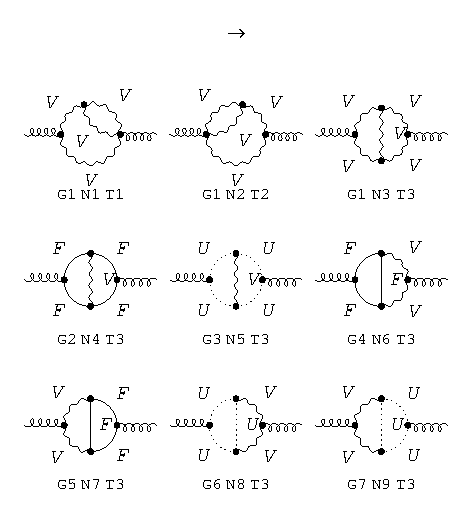
\includegraphics{qcd2loopgluon-tex_gr1}}
\scalebox{1.0}{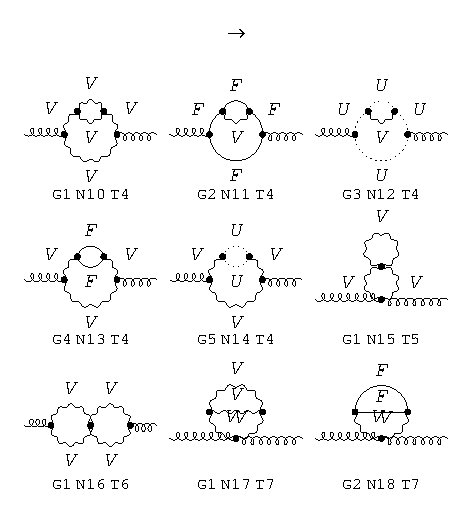
\includegraphics{qcd2loopgluon-tex_gr2}}
\scalebox{1.0}{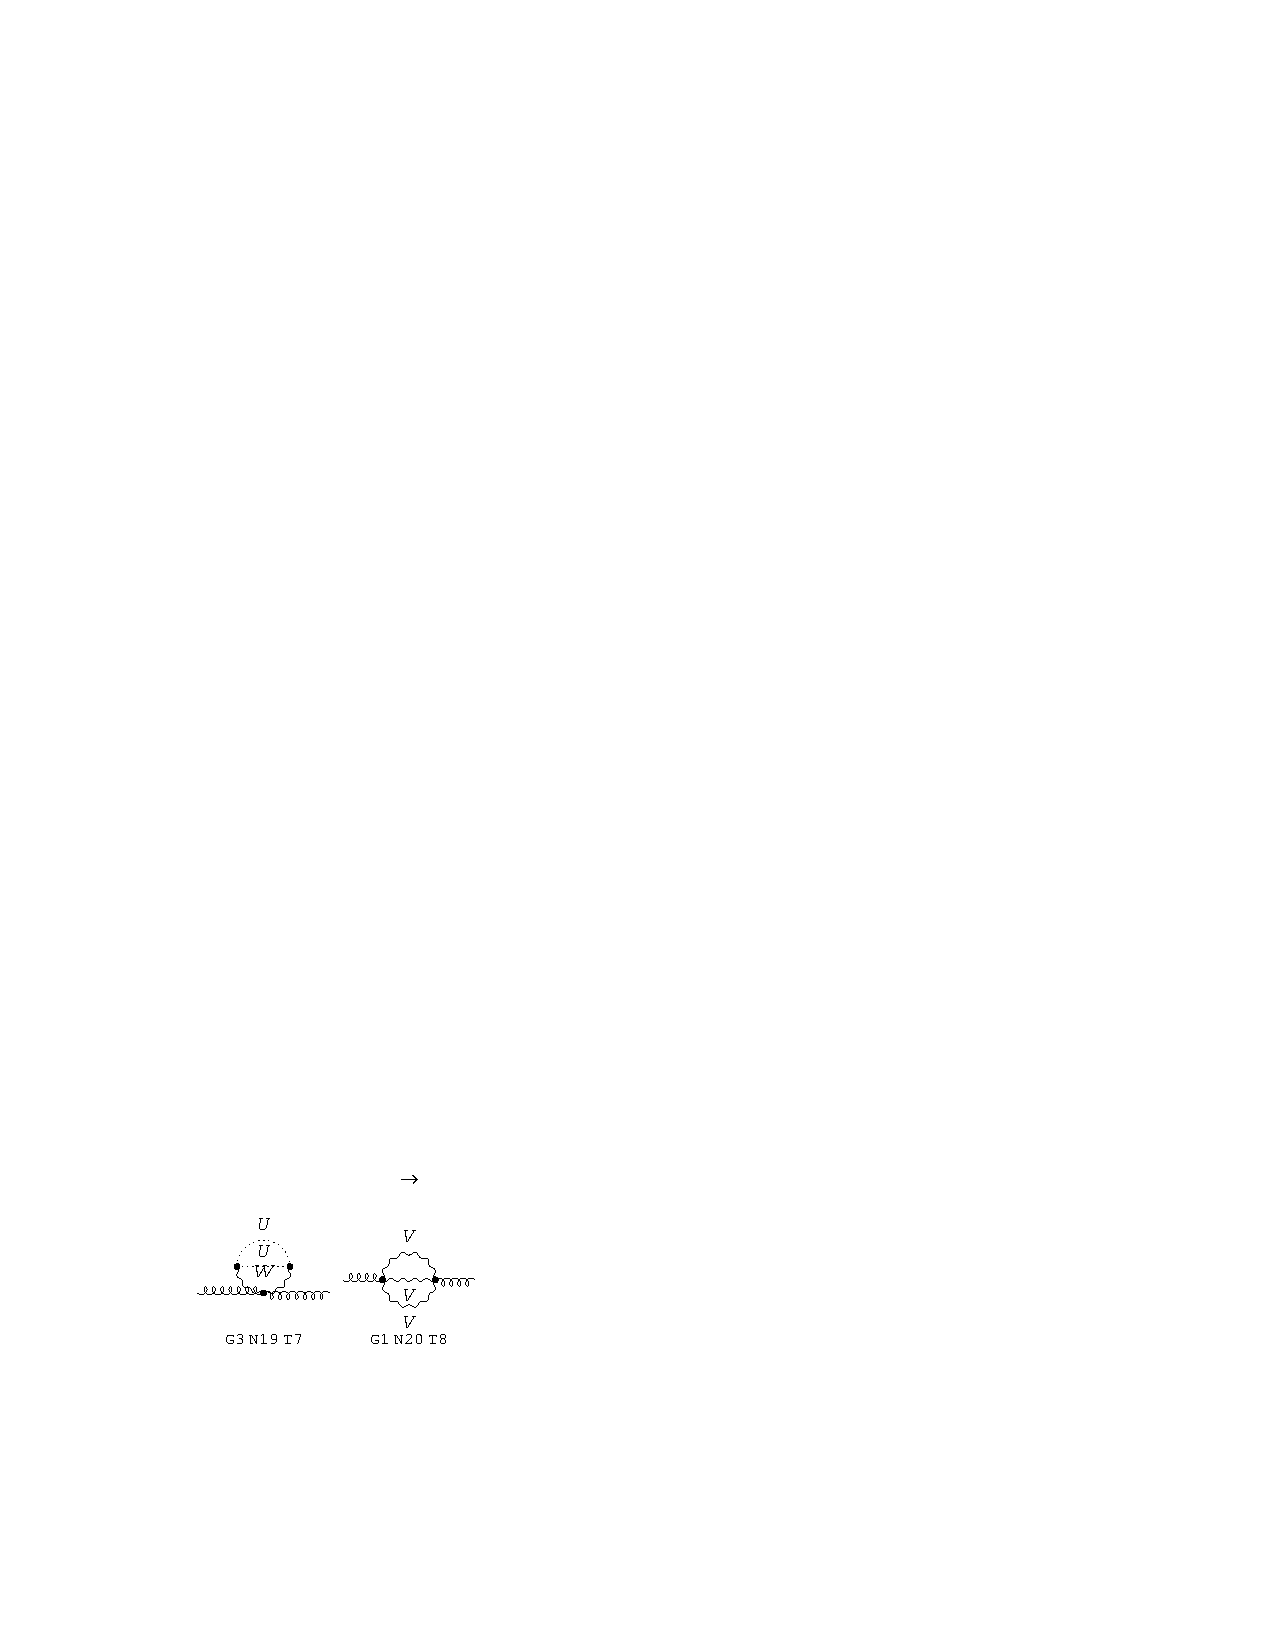
\includegraphics{qcd2loopgluon-tex_gr3}}
\caption{2-loop gluon self-energy diagrams.}
\end{center}
\end{figure}

\Subsubsection*{Calculating the bare 2-loop on-shell gluon selfenergy diagrams}

In the Model file all incoming momenta are specificied by p1, p2, ... and all outgoing by k1, k2, ... .\\
We substitute p1 to p and k1 to -p and do some further substitutions.

\dispSFinmath{
\MathBegin{MathArray}{l}
\Mvariable{amps}=\Muserfunction{CreateFeynAmp}[
       \Mvariable{inserts},\Mvariable{Truncated}\rightarrow \Mvariable{True},\Mvariable{PreFactor}\rightarrow 1]/.
      \Mvariable{k1}\rightarrow -\Mvariable{p1}/.\Mvariable{p1}\rightarrow p/.  \\
\noalign{\vspace{0.555556ex}}
\hspace{3.em} 
          \Muserfunction{FeynAmpList}[\_\_]\RuleDelayed \Mvariable{List}\multsp /.\multsp 
      \Muserfunction{FeynAmp}[\_,\_,\Mvariable{x\_}]\RuleDelayed x;;\\
\MathEnd{MathArray}
}

\dispSFinmath{
\Muserfunction{amps}[[3]]
}

\dispSFoutmath{
\MathBegin{MathArray}{l}
\frac{1}{2}\multsp \Pi _{g}^{\Mvariable{li9}\Mvariable{li10}}(p-{q_1})\multsp 
   \Pi _{g}^{\Mvariable{li3}\Mvariable{li4}}({q_1})\multsp \Pi _{g}^{\Mvariable{li11}\Mvariable{li12}}(-p-{q_2})\multsp 
   \Pi _{g}^{\Mvariable{li5}\Mvariable{li6}}({q_2})\multsp \Pi _{g}^{\Mvariable{li7}\Mvariable{li8}}({q_1}+{q_2})\multsp 
   {V^{\Mvariable{li1}\Mvariable{li4}\Mvariable{li10}}}(p,\multsp {q_1},\multsp p-{q_1})\multsp 
   {V^{\Mvariable{li2}\Mvariable{li6}\Mvariable{li12}}}(p,\multsp {q_2},\multsp -p-{q_2})\multsp   \\
\noalign{\vspace{0.840278ex}}
   \hspace{1.em} {V^{\Mvariable{li3}\Mvariable{li5}\Mvariable{li8}}}(-{q_1},\multsp -{q_2},\multsp {q_1}+{q_2})\multsp 
   {V^{\Mvariable{li7}\Mvariable{li9}\Mvariable{li11}}}(-{q_1}-{q_2},\multsp {q_1}-p,\multsp p+{q_2})\multsp 
   {f_{\Mvariable{ci1}\Mvariable{ci4}\Mvariable{ci10}}}\multsp {f_{\Mvariable{ci2}\Mvariable{ci5}\Mvariable{ci11}}}\multsp 
   {f_{\Mvariable{ci4}\Mvariable{ci5}\Mvariable{ci8}}}\multsp {f_{\Mvariable{ci8}\Mvariable{ci10}\Mvariable{ci11}}}\\
\MathEnd{MathArray}
}

\dispSFinmath{
\Mvariable{amp31}=\Muserfunction{amps}[[3]]/.\Mvariable{q2}\rightarrow -\Mvariable{q2}
}

\dispSFoutmath{
\MathBegin{MathArray}{l}
\frac{1}{2}\multsp \Pi _{g}^{\Mvariable{li9}\Mvariable{li10}}(p-{q_1})\multsp 
   \Pi _{g}^{\Mvariable{li3}\Mvariable{li4}}({q_1})\multsp \Pi _{g}^{\Mvariable{li7}\Mvariable{li8}}({q_1}-{q_2})\multsp 
   \Pi _{g}^{\Mvariable{li5}\Mvariable{li6}}({q_2})\multsp \Pi _{g}^{\Mvariable{li11}\Mvariable{li12}}({q_2}-p)\multsp 
   {V^{\Mvariable{li1}\Mvariable{li4}\Mvariable{li10}}}(p,\multsp {q_1},\multsp p-{q_1})\multsp 
   {V^{\Mvariable{li2}\Mvariable{li6}\Mvariable{li12}}}(p,\multsp -{q_2},\multsp {q_2}-p)\multsp   \\
\noalign{\vspace{0.840278ex}}
   \hspace{1.em} {V^{\Mvariable{li3}\Mvariable{li5}\Mvariable{li8}}}(-{q_1},\multsp {q_2},\multsp {q_1}-{q_2})\multsp 
   {V^{\Mvariable{li7}\Mvariable{li9}\Mvariable{li11}}}({q_2}-{q_1},\multsp {q_1}-p,\multsp p-{q_2})\multsp 
   {f_{\Mvariable{ci1}\Mvariable{ci4}\Mvariable{ci10}}}\multsp {f_{\Mvariable{ci2}\Mvariable{ci5}\Mvariable{ci11}}}\multsp 
   {f_{\Mvariable{ci4}\Mvariable{ci5}\Mvariable{ci8}}}\multsp {f_{\Mvariable{ci8}\Mvariable{ci10}\Mvariable{ci11}}}\\
\MathEnd{MathArray}
}

\dispSFinmath{
\Muserfunction{amp31}//\Mfunction{InputForm}
}

\dispSFoutmath{
\MathBegin{MathArray}{l}
(\Muserfunction{GluonPropagator}[
     p\multsp -\multsp \Mvariable{q1},\multsp \{\Mvariable{li9}\},\multsp \{\Mvariable{li10}\}]*  \\
\noalign{\vspace{0.625ex}}\multsp
    \multsp \Muserfunction{GluonPropagator}[\Mvariable{q1},\multsp \{\Mvariable{li3}\},\multsp \{\Mvariable{li4}\}]*  \\
   \noalign{\vspace{0.625ex}}\multsp \multsp \Muserfunction{GluonPropagator}[
    \Mvariable{q1}\multsp -\multsp \Mvariable{q2},\multsp \{\Mvariable{li7}\},\multsp \{\Mvariable{li8}\}]*  \\
   \noalign{\vspace{0.625ex}}\multsp \multsp \Muserfunction{GluonPropagator}[
    \Mvariable{q2},\multsp \{\Mvariable{li5}\},\multsp \{\Mvariable{li6}\}]*  \\
\noalign{\vspace{0.625ex}}\multsp \multsp 
   \Muserfunction{GluonPropagator}[-p\multsp +\multsp \Mvariable{q2},\multsp \{\Mvariable{li11}\},\multsp \{\Mvariable{li12}\}]*  \\
   \noalign{\vspace{0.625ex}}\multsp \multsp \Muserfunction{GluonVertex}[
    \{p,\multsp \Mvariable{li1}\},\multsp \{\Mvariable{q1},\multsp \Mvariable{li4}\},\multsp 
     \{p\multsp -\multsp \Mvariable{q1},\multsp \Mvariable{li10}\}]*  \\
\noalign{\vspace{0.625ex}}\multsp \multsp 
   \Muserfunction{GluonVertex}[\{p,\multsp \Mvariable{li2}\},\multsp \{-\Mvariable{q2},\multsp \Mvariable{li6}\},\multsp 
     \{-p\multsp +\multsp \Mvariable{q2},\multsp \Mvariable{li12}\}]*  \\
\noalign{\vspace{0.625ex}}\multsp \multsp 
   \Muserfunction{GluonVertex}[\{-\Mvariable{q1},\multsp \Mvariable{li3}\},\multsp \{\Mvariable{q2},\multsp \Mvariable{li5}\},\multsp 
     \{\Mvariable{q1}\multsp -\multsp \Mvariable{q2},\multsp \Mvariable{li8}\}]*  \\
\noalign{\vspace{0.625ex}}\multsp \multsp 
   \Muserfunction{GluonVertex}[\{-\Mvariable{q1}\multsp +\multsp \Mvariable{q2},\multsp \Mvariable{li7}\},\multsp 
     \{-p\multsp +\multsp \Mvariable{q1},\multsp \Mvariable{li9}\},\multsp   \\
\noalign{\vspace{0.625ex}}\multsp \multsp \multsp 
     \{p\multsp -\multsp \Mvariable{q2},\multsp \Mvariable{li11}\}]*
   \Muserfunction{SUNF}[\Mvariable{ci1},\multsp \Mvariable{ci4},\multsp \Mvariable{ci10}]*  \\
\noalign{\vspace{0.625ex}}\multsp \multsp 
   \Muserfunction{SUNF}[\Mvariable{ci2},\multsp \Mvariable{ci5},\multsp \Mvariable{ci11}]*
   \Muserfunction{SUNF}[\Mvariable{ci4},\multsp \Mvariable{ci5},\multsp \Mvariable{ci8}]*  \\
\noalign{\vspace{0.625ex}}\multsp \multsp 
     \Muserfunction{SUNF}[\Mvariable{ci8},\multsp \Mvariable{ci10},\multsp \Mvariable{ci11}])/2\\
\MathEnd{MathArray}
}

\dispSFinmath{
\Mvariable{amp32}=\Muserfunction{SUNSimplify}[\Mvariable{Explicit}@\multsp \Mvariable{amp31}]
}

\dispSFoutmath{
\MathBegin{MathArray}{l}
-\big(\ImaginaryI \multsp C_{A}^{2}\multsp {g^{\Mvariable{li10}\Mvariable{li9}}}\multsp 
     {g^{\Mvariable{li11}\Mvariable{li12}}}\multsp {g^{\Mvariable{li3}\Mvariable{li4}}}\multsp 
     \big(-{p^{\Mvariable{li1}}}\multsp {g^{\Mvariable{li10}\Mvariable{li4}}}+
       2\multsp q_{1}^{\Mvariable{li1}}\multsp {g^{\Mvariable{li10}\Mvariable{li4}}}+
       {g^{\Mvariable{li1}\Mvariable{li4}}}\multsp {p^{\Mvariable{li10}}}-
       {g^{\Mvariable{li1}\Mvariable{li4}}}\multsp q_{1}^{\Mvariable{li10}}-
       {g^{\Mvariable{li1}\Mvariable{li10}}}\multsp q_{1}^{\Mvariable{li4}}\big)\multsp   \\
\noalign{\vspace{0.659722ex}}
   \hspace{4.em} {g^{\Mvariable{li5}\Mvariable{li6}}}\multsp 
   \big({p^{\Mvariable{li12}}}\multsp {g^{\Mvariable{li2}\Mvariable{li6}}}+
     q_{2}^{\Mvariable{li12}}\multsp {g^{\Mvariable{li2}\Mvariable{li6}}}+
     {g^{\Mvariable{li12}\Mvariable{li6}}}\multsp {p^{\Mvariable{li2}}}-
     2\multsp {g^{\Mvariable{li12}\Mvariable{li6}}}\multsp q_{2}^{\Mvariable{li2}}-
     2\multsp {g^{\Mvariable{li12}\Mvariable{li2}}}\multsp {p^{\Mvariable{li6}}}+
     {g^{\Mvariable{li12}\Mvariable{li2}}}\multsp q_{2}^{\Mvariable{li6}}\big)\multsp   \\
\noalign{\vspace{0.659722ex}}
   \hspace{4.em} {g^{\Mvariable{li7}\Mvariable{li8}}}\multsp 
   \big(-q_{1}^{\Mvariable{li3}}\multsp {g^{\Mvariable{li5}\Mvariable{li8}}}+
     2\multsp q_{2}^{\Mvariable{li3}}\multsp {g^{\Mvariable{li5}\Mvariable{li8}}}+
     2\multsp {g^{\Mvariable{li3}\Mvariable{li8}}}\multsp q_{1}^{\Mvariable{li5}}-
     {g^{\Mvariable{li3}\Mvariable{li8}}}\multsp q_{2}^{\Mvariable{li5}}-
     {g^{\Mvariable{li3}\Mvariable{li5}}}\multsp q_{1}^{\Mvariable{li8}}-
     {g^{\Mvariable{li3}\Mvariable{li5}}}\multsp q_{2}^{\Mvariable{li8}}\big)\multsp   \\
\noalign{\vspace{0.659722ex}}
   \hspace{4.em} \big({p^{\Mvariable{li11}}}\multsp {g^{\Mvariable{li7}\Mvariable{li9}}}-
     2\multsp q_{1}^{\Mvariable{li11}}\multsp {g^{\Mvariable{li7}\Mvariable{li9}}}+
     q_{2}^{\Mvariable{li11}}\multsp {g^{\Mvariable{li7}\Mvariable{li9}}}-
     2\multsp {g^{\Mvariable{li11}\Mvariable{li9}}}\multsp {p^{\Mvariable{li7}}}+
     {g^{\Mvariable{li11}\Mvariable{li9}}}\multsp q_{1}^{\Mvariable{li7}}+
     {g^{\Mvariable{li11}\Mvariable{li9}}}\multsp q_{2}^{\Mvariable{li7}}+
     {g^{\Mvariable{li11}\Mvariable{li7}}}\multsp {p^{\Mvariable{li9}}}+
     {g^{\Mvariable{li11}\Mvariable{li7}}}\multsp q_{1}^{\Mvariable{li9}}-
     2\multsp {g^{\Mvariable{li11}\Mvariable{li7}}}\multsp q_{2}^{\Mvariable{li9}}\big)\multsp   \\
\noalign{\vspace{0.659722ex}}
   \hspace{4.em} {{\delta }_{\Mvariable{ci1}\Mvariable{ci2}}}\big)\big/
   \big(4\multsp {{(p-{q_1})}^2}\multsp q_{1}^{2}\multsp {{({q_1}-{q_2})}^2}\multsp q_{2}^{2}\multsp {{({q_2}-p)}^2}\big)\\
   \MathEnd{MathArray}
}

\dispSFinmath{
\MathBegin{MathArray}{l}
\Mvariable{Timing}[  \\
\noalign{\vspace{0.555556ex}}
\hspace{1.em} \Mvariable{amp33}=  \\
   \noalign{\vspace{0.555556ex}}
\hspace{2.em} \Muserfunction{Collect2}[\Mvariable{FeynAmpDenominatorCombine}@  \\
\noalign{\vspace{
   0.555556ex}}
\hspace{4.em} \Muserfunction{Contract3}[
         \Muserfunction{Explicit}[\Mvariable{amp32}]/.\Mvariable{li1}\rightarrow \Mvariable{li2}/.
          \Muserfunction{SUNDelta}[\_\_]\RuleDelayed 1],\Mvariable{q1},\Mvariable{q2}];]\\
\MathEnd{MathArray}
}

\dispSFoutmath{
\{0.71\multsp \Mvariable{Second},\Mvariable{Null}\}
}

\dispSFinmath{
\Mvariable{amp33}
}

\dispSFoutmath{
\MathBegin{MathArray}{l}
-\frac{\ImaginaryI \multsp C_{A}^{2}\multsp (11-5\multsp D)\multsp {{p\cdot {q_1}}^2}}
     {2\multsp q_{1}^{2}.q_{2}^{2}.{{(p-{q_1})}^2}.{{({q_2}-p)}^2}.{{({q_1}-{q_2})}^2}}-
   \frac{\ImaginaryI \multsp C_{A}^{2}\multsp (5-2\multsp D)\multsp {{{q_1}\cdot {q_2}}^2}}
    {2\multsp q_{1}^{2}.q_{2}^{2}.{{(p-{q_1})}^2}.{{({q_2}-p)}^2}.{{({q_1}-{q_2})}^2}}-  \\
\noalign{\vspace{1.47917ex}}
   \hspace{1.em} \frac{3\multsp \ImaginaryI \multsp C_{A}^{2}\multsp (1-D)\multsp {p^2}\multsp p\cdot {q_1}}
    {2\multsp q_{1}^{2}.q_{2}^{2}.{{(p-{q_1})}^2}.{{({q_2}-p)}^2}.{{({q_1}-{q_2})}^2}}+
   \frac{\ImaginaryI \multsp C_{A}^{2}\multsp (34-19\multsp D)\multsp p\cdot {q_1}\multsp p\cdot {q_2}}
    {2\multsp q_{1}^{2}.q_{2}^{2}.{{(p-{q_1})}^2}.{{({q_2}-p)}^2}.{{({q_1}-{q_2})}^2}}+
   \frac{\ImaginaryI \multsp C_{A}^{2}\multsp (7-4\multsp D)\multsp {p^2}\multsp q_{1}^{2}}
    {q_{1}^{2}.q_{2}^{2}.{{(p-{q_1})}^2}.{{({q_2}-p)}^2}.{{({q_1}-{q_2})}^2}}-  \\
\noalign{\vspace{1.47917ex}}
\hspace{1.em} \frac{
       \ImaginaryI \multsp C_{A}^{2}\multsp (14-11\multsp D)\multsp p\cdot {q_2}\multsp q_{1}^{2}}{2\multsp 
      q_{1}^{2}.q_{2}^{2}.{{(p-{q_1})}^2}.{{({q_2}-p)}^2}.{{({q_1}-{q_2})}^2}}-
   \frac{5\multsp \ImaginaryI \multsp C_{A}^{2}\multsp (5-2\multsp D)\multsp {p^2}\multsp {q_1}\cdot {q_2}}
    {2\multsp q_{1}^{2}.q_{2}^{2}.{{(p-{q_1})}^2}.{{({q_2}-p)}^2}.{{({q_1}-{q_2})}^2}}+
   \frac{\ImaginaryI \multsp C_{A}^{2}\multsp (5-2\multsp D)\multsp p\cdot {q_1}\multsp {q_1}\cdot {q_2}}
    {2\multsp q_{1}^{2}.q_{2}^{2}.{{(p-{q_1})}^2}.{{({q_2}-p)}^2}.{{({q_1}-{q_2})}^2}}+  \\
\noalign{\vspace{1.47917ex}}
   \hspace{1.em} \frac{\ImaginaryI \multsp C_{A}^{2}\multsp (5-2\multsp D)\multsp p\cdot {q_2}\multsp {q_1}\cdot {q_2}}
    {2\multsp q_{1}^{2}.q_{2}^{2}.{{(p-{q_1})}^2}.{{({q_2}-p)}^2}.{{({q_1}-{q_2})}^2}}-
   \frac{\ImaginaryI \multsp C_{A}^{2}\multsp (14-11\multsp D)\multsp p\cdot {q_1}\multsp q_{2}^{2}}
    {2\multsp q_{1}^{2}.q_{2}^{2}.{{(p-{q_1})}^2}.{{({q_2}-p)}^2}.{{({q_1}-{q_2})}^2}}+
   \frac{\ImaginaryI \multsp C_{A}^{2}\multsp (14-11\multsp D)\multsp q_{1}^{2}\multsp q_{2}^{2}}
    {2\multsp q_{1}^{2}.q_{2}^{2}.{{(p-{q_1})}^2}.{{({q_2}-p)}^2}.{{({q_1}-{q_2})}^2}}\\
\MathEnd{MathArray}
}

\dispSFinmath{
\Mvariable{amp34}=\Muserfunction{ToTFi}[\Mvariable{amp33},\Mvariable{q1},\Mvariable{q2},p]//\Muserfunction{FCE}
}

\dispSFoutmath{
\MathBegin{MathArray}{l}
-\frac{5}{2}\multsp \ImaginaryI \multsp (5-2\multsp D)\multsp {p^2}\multsp 
    F_{\{1,0\}\{1,0\}\{1,0\}\{1,0\}\{1,0\}}^{(D)\multsp 00001}\multsp C_{A}^{2}-
   \frac{1}{2}\multsp \ImaginaryI \multsp (5-2\multsp D)\multsp F_{\{1,0\}\{1,0\}\{1,0\}\{1,0\}\{1,0\}}^{(D)\multsp 00002}\multsp 
    C_{A}^{2}+  \\
\noalign{\vspace{1.10417ex}}
\hspace{1.em} \frac{1}{2}\multsp \ImaginaryI \multsp (5-2\multsp D)\multsp 
    F_{\{1,0\}\{1,0\}\{1,0\}\{1,0\}\{1,0\}}^{(D)\multsp 00011}\multsp C_{A}^{2}-
   \frac{3}{2}\multsp \ImaginaryI \multsp (1-D)\multsp {p^2}\multsp F_{\{1,0\}\{1,0\}\{1,0\}\{1,0\}\{1,0\}}^{(D)\multsp 00100}\multsp 
    C_{A}^{2}+\frac{1}{2}\multsp \ImaginaryI \multsp (5-2\multsp D)\multsp F_{\{1,0\}\{1,0\}\{1,0\}\{1,0\}\{1,0\}}^{(D)\multsp 00101}
    \multsp C_{A}^{2}+  \\
\noalign{\vspace{1.10417ex}}
\hspace{1.em} \frac{1}{2}\multsp \ImaginaryI \multsp (34-19\multsp D)\multsp 
    F_{\{1,0\}\{1,0\}\{1,0\}\{1,0\}\{1,0\}}^{(D)\multsp 00110}\multsp C_{A}^{2}-
   \frac{1}{2}\multsp \ImaginaryI \multsp (11-5\multsp D)\multsp F_{\{1,0\}\{1,0\}\{1,0\}\{1,0\}\{1,0\}}^{(D)\multsp 00200}\multsp 
    C_{A}^{2}-\frac{1}{2}\multsp \ImaginaryI \multsp (14-11\multsp D)\multsp F_{\{1,0\}\{1,0\}\{1,0\}\{1,0\}\{1,0\}}^{(D)\multsp 01100}
    \multsp C_{A}^{2}+  \\
\noalign{\vspace{1.10417ex}}
\hspace{1.em} \ImaginaryI \multsp (7-4\multsp D)\multsp {p^2}\multsp 
    F_{\{1,0\}\{1,0\}\{1,0\}\{1,0\}\{1,0\}}^{(D)\multsp 10000}\multsp C_{A}^{2}-
   \frac{1}{2}\multsp \ImaginaryI \multsp (14-11\multsp D)\multsp F_{\{1,0\}\{1,0\}\{1,0\}\{1,0\}\{1,0\}}^{(D)\multsp 10010}\multsp 
    C_{A}^{2}+\frac{1}{2}\multsp \ImaginaryI \multsp (14-11\multsp D)\multsp F_{\{1,0\}\{1,0\}\{1,0\}\{1,0\}\{1,0\}}^{(D)\multsp 11000}
    \multsp C_{A}^{2}\\
\MathEnd{MathArray}
}

\dispSFinmath{
\Mvariable{amp35}=\Muserfunction{TarcerRecurse}[\Mvariable{amp34}]
}

\dispSFoutmath{
-\frac{\ImaginaryI \multsp (2\multsp {D^2}-57\multsp D+136)\multsp {p^2}\multsp {{B_{\{1,0\}\{1,0\}}^{(D)}}^2}\multsp C_{A}^{2}}
     {16\multsp (D-4)}-\frac{\ImaginaryI \multsp (2\multsp {D^3}+19\multsp {D^2}-124\multsp D+184)\multsp J_{\{1,0\}\{1,0\}\{1,0\}}^{(D)}
      \multsp C_{A}^{2}}{4\multsp {{(D-4)}^2}}
}


